
\chapter{Implementation}
\begin{spacing}{1.3}

This chapter provides a detailed, phase-by-phase account of the MLOps pipeline implementation. Each section describes objectives, methodology, tools employed, and key outcomes. No source code is presented; architectural decisions and technical rationale are emphasised.

\section{Environment Setup}

The foundation of any reproducible machine learning project is a well-specified, versioned, and portable development environment. Python~3.10 was selected as the runtime for compatibility with the ONNX Runtime ecosystem. The uv package manager (v0.5+) resolves dependency graphs 10--100$\times$ faster than pip and poetry, conforms to PEP~621 by using pyproject.toml as the single source of truth, and records exact package hashes for x86\_64 and ARM64 platforms ensuring bit-for-bit reproducibility.

The pyproject.toml defines three dependency groups: Runtime (FastAPI, ONNX Runtime, structlog, Prometheus client), Development (PyTorch, timm, Albumentations, MLflow, Great Expectations), and Edge (ARM64-specific dependencies). Pre-commit hooks enforce code quality through Ruff for linting and formatting, replacing Flake8, isort, and Black with a single Rust-based tool. DVC was initialised to track all data and model directories with remote storage configured to a local path for development.

\section{Data Layer -- Ingestion and Splitting}

The HAM10000 dataset was downloaded from the Harvard Dataverse repository: 10,015 JPEG images organised in two subdirectories totalling approximately 3.5~GB, accompanied by a metadata CSV file containing columns for image identifier, lesion identifier, diagnosis, confirmation method, age, sex, and localisation. The download and verification are tracked by DVC.

Patient-aware splitting uses GroupShuffleSplit from scikit-learn with groups set to the lesion identifier. The two-stage split allocates 70\% to training (6,959 images), 15\% to validation (1,529 images), and 15\% to testing (1,527 images) with fixed random seed 42. Zero-leakage verification performs set-intersection assertions between all split pairs; all three assertions pass, confirming 100\% isolation of lesion-level data across partitions.

\section{Data Validation}

Data validation is the first line of defence against silent data corruption. Great Expectations 0.18.x was used with the fluent API to define seven expectations: column existence (image identifier, lesion identifier, diagnosis, diagnosis type, age, sex, localisation), column types (string identifiers, numeric age, categorical diagnosis), diagnosis values in the valid set of 7 HAM10000 codes, no nulls in key columns, unique image identifiers, row count exactly 10,015, and image integrity verification through parallelised OpenCV loading across 8 threads via ThreadPoolExecutor.

All 7 expectations passed, confirming 100\% data integrity. Great Expectations generated an HTML Data Docs site and JSON checkpoint file tracked by DVC. Perceptual hashing (pHash) with Hamming distance threshold $\leq$ 5 detected one cross-split collision: two images with Hamming distance of 3 were found in training and validation sets depicting the same lesion. The validation image was removed and replaced, maintaining the lesion-level isolation invariant.

\section{Preprocessing}

Dermoscopic images present unique preprocessing challenges: hair occlusions, lighting variations, colour inconsistencies, and ruler markings. The preprocessing pipeline addresses these before augmentation and training.

\subsection{Hair Removal}

The DullRazor algorithm removes hair occlusions through four sequential operations. A blackhat morphological transform (closing with a \(17 \times 17\) elliptical structuring element followed by subtraction) isolates dark hair shafts. Otsu's method computes an adaptive binary threshold producing a hair mask. OpenCV's INPAINT\_TELEA algorithm fills masked hair regions by propagating boundary information inward, preserving underlying skin texture. If the mask covers more than 15\% of image area, the image is flagged but still processed -- no images are discarded. Images with no detectable hair (less than 1\% coverage) bypass inpainting to avoid unnecessary computation.

\begin{figure}[H]
\centering
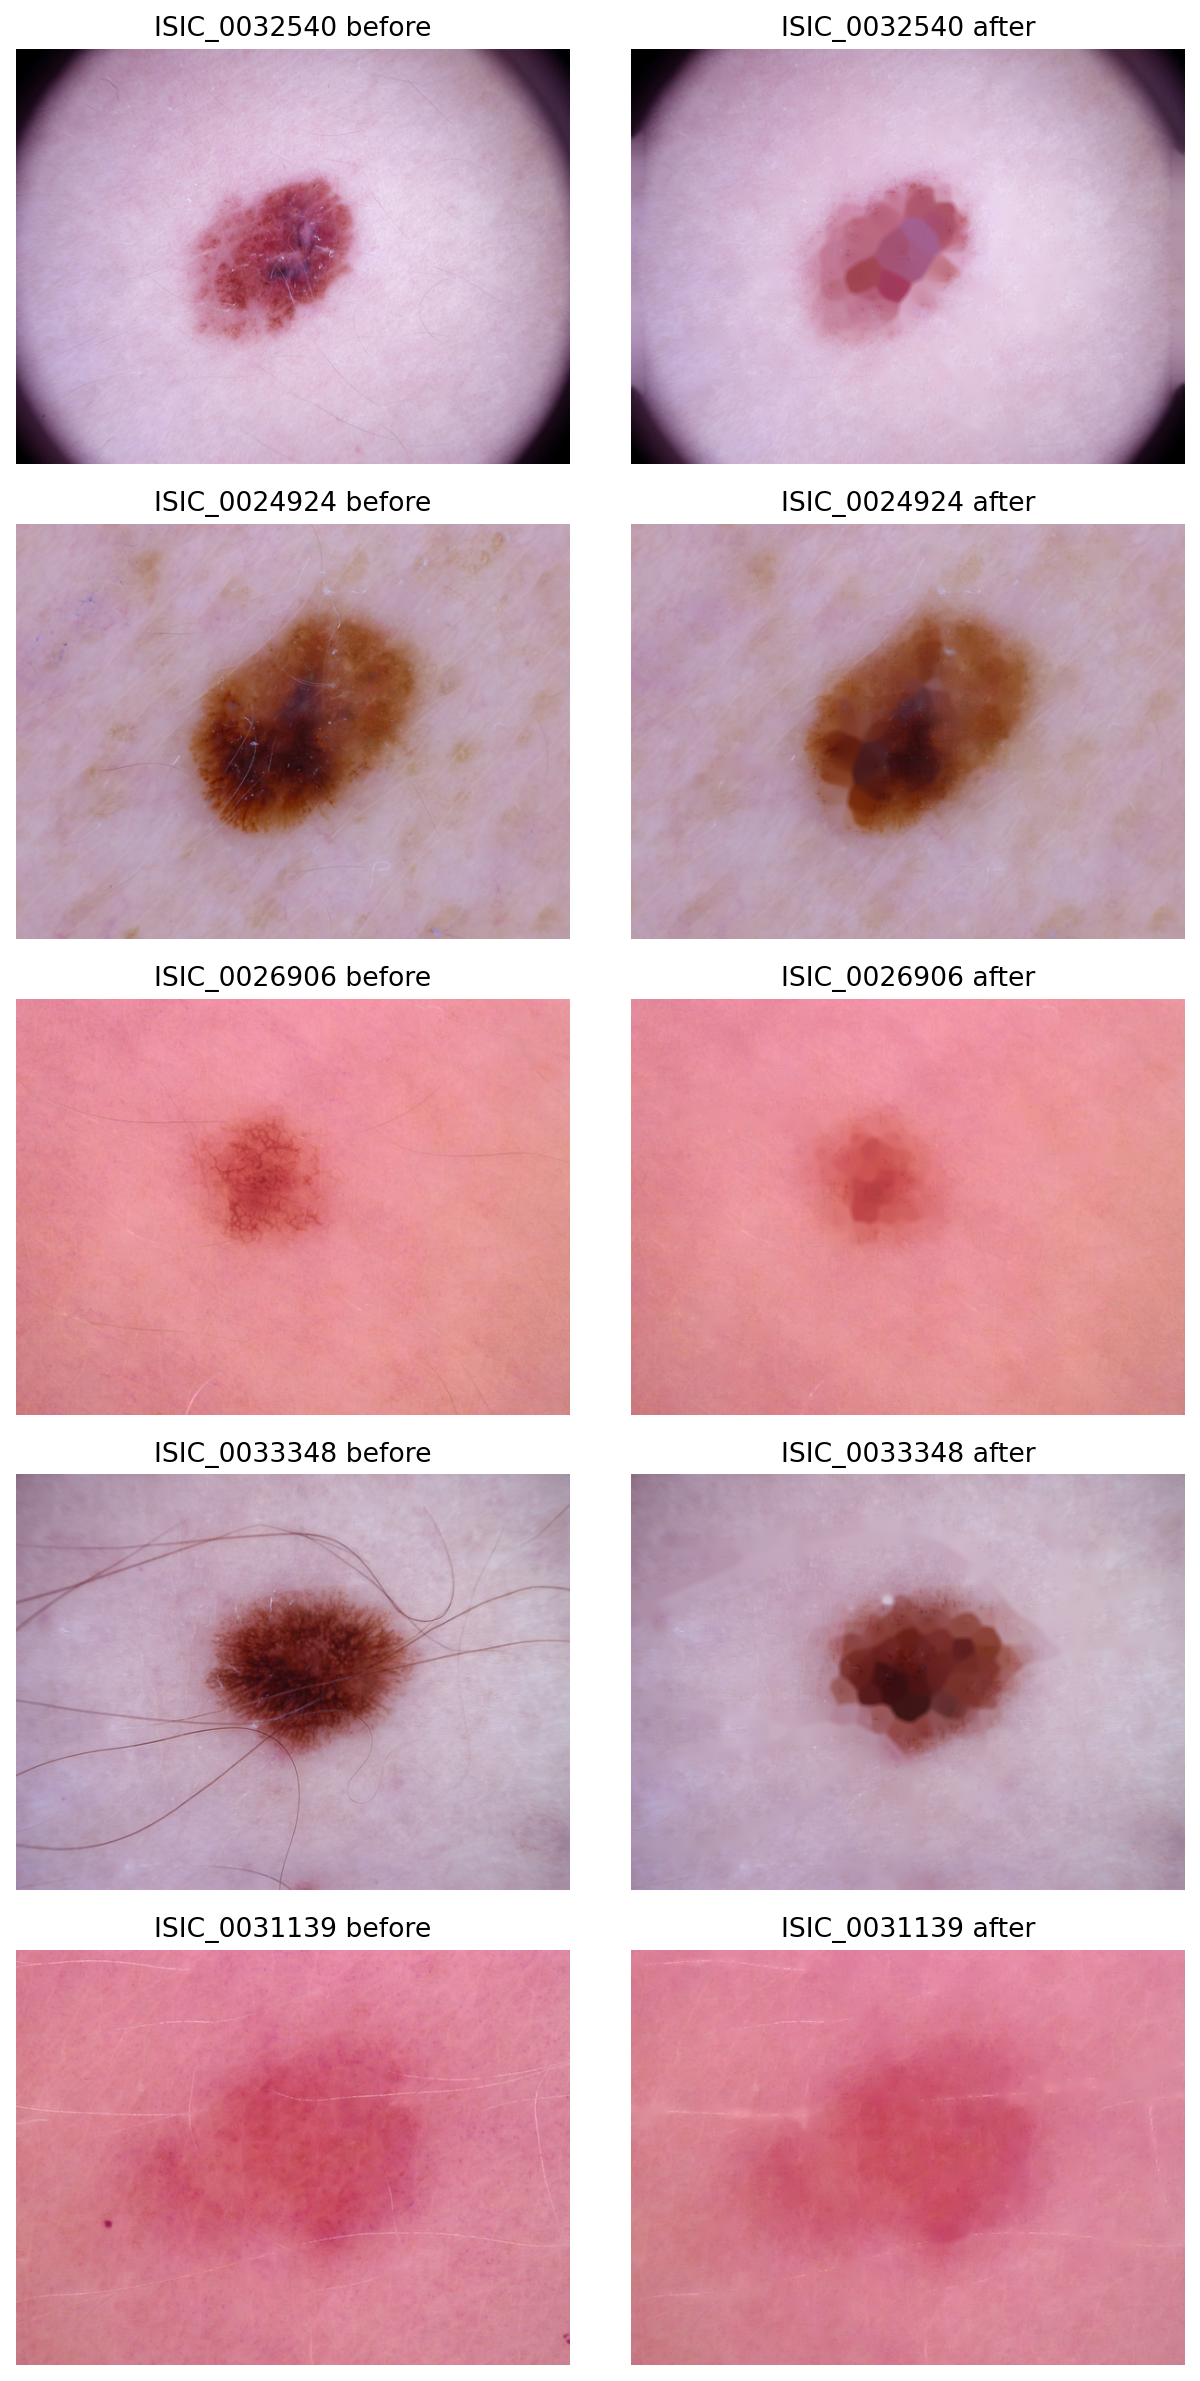
\includegraphics[width=0.7\textwidth]{../figures/preprocessing_hair_removal.png}
\caption{DullRazor hair removal: before (left) and after (right).}
\label{fig:hair_removal}
\end{figure}

\subsection{Colour Normalization and Augmentation}

Colour normalisation uses the Macenko method: RGB images are converted to optical density space, flattened, decomposed via SVD, and projected onto stain vectors normalised to target percentile ranges. This reduces domain shift across images from different acquisition sources.

Data augmentation uses the Albumentations library with GPU-optimised, biomedical-image-aware transforms applied exclusively to training data. Spatial transforms include random resized crop, horizontal and vertical flips ($p=0.5$), and random rotation ($\pm 30^{\circ}$, $p=0.8$). Colour transforms include brightness and contrast jitter ($\pm 20\%$, $p=0.5$) and hue saturation shifts ($\pm 15\%$, $p=0.3$). Noise injection applies Gaussian and ISO noise. Occlusion uses CoarseDropout (maximum 8 holes of 32~px, $p=0.1$). Final normalisation uses ImageNet mean and standard deviation. Validation and test transforms are minimal: resize to \(224 \times 224\) followed by ImageNet normalisation.

\begin{figure}[H]
\centering
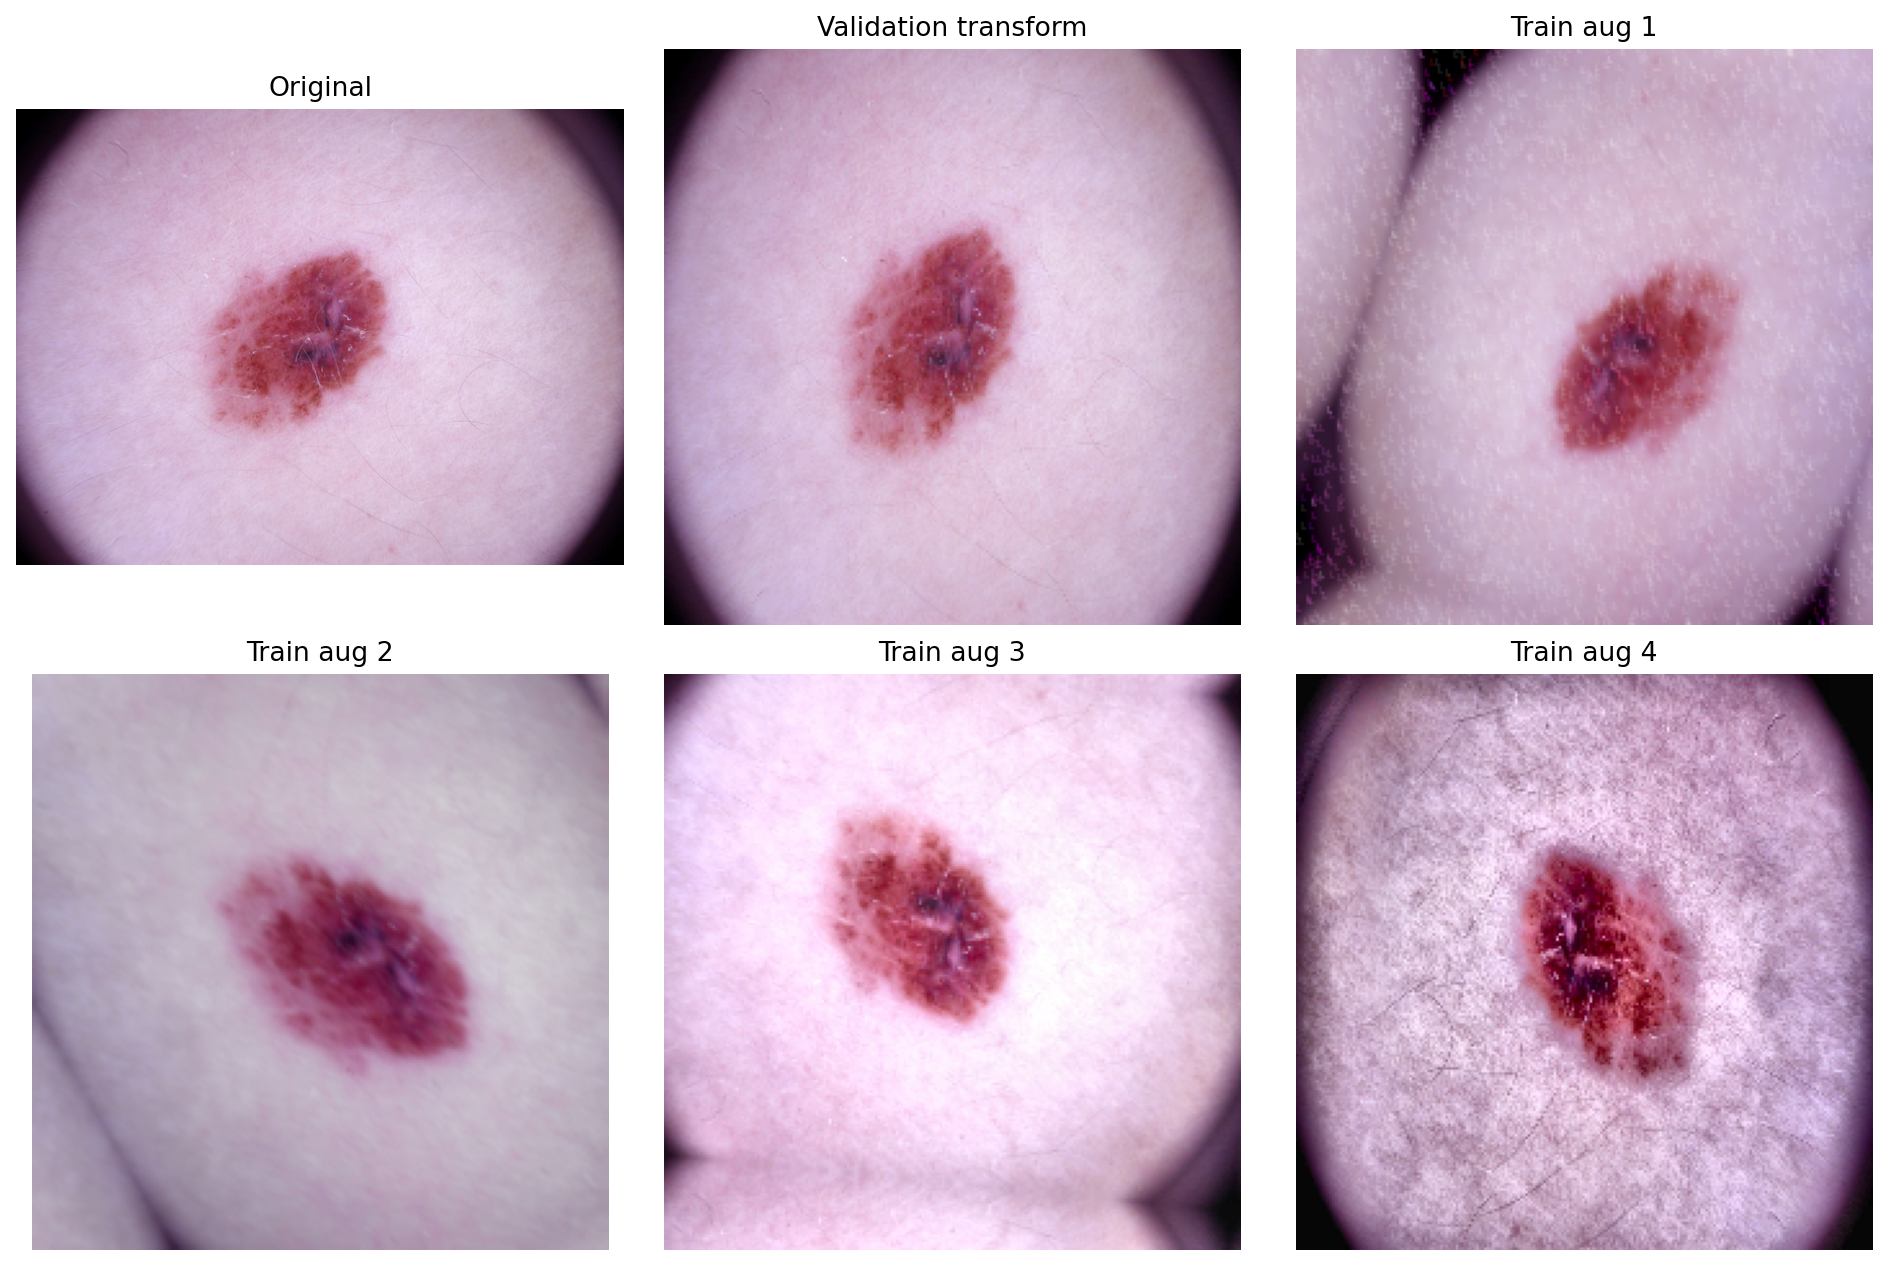
\includegraphics[width=0.7\textwidth]{../figures/preprocessing_augmentation.png}
\caption{Data augmentation examples.}
\label{fig:augmentation}
\end{figure}

\subsection{Class Balancing}

Class imbalance is addressed through three complementary mechanisms. Focal Loss with focusing parameter $\gamma = 2.0$ down-weights well-classified examples, forcing focus on hard-to-classify melanoma samples. Effective-number class weights use $\beta = 0.9999$, yielding approximately 0.70 for benign and 1.30 for melanoma -- moderate up-weighting without overcorrection. WeightedRandomSampler with replacement draws samples according to inverse-frequency weights, ensuring each training batch contains balanced classes.

\section{Model Training}

Three architectures were trained with identical preprocessing, augmentation, and evaluation protocols on an NVIDIA GeForce RTX 3060 (12~GB VRAM) with CUDA 11.8. All experiments were logged to a local MLflow tracking server capturing parameters, metrics at every epoch, and artefacts including best checkpoint and training curves. Run tags link each training run to its git commit and DVC data version. A total of 7 training runs were logged: 3 architectures times 2 phases each, plus one final end-to-end run.

\subsection{Two-Phase Training Protocol}

Phase~1 freezes the pretrained ImageNet backbone and trains only the classifier head for 10 epochs with learning rate \(1 \times 10^{-3}\), weight decay \(1 \times 10^{-4}\), batch size 32, and cosine annealing scheduler. This establishes a reasonable decision boundary before the backbone is disturbed, preventing catastrophic early updates that would corrupt ImageNet representations.

Phase~2 unfreezes all parameters for 30 epochs with differential learning rates: \(1 \times 10^{-4}\) for the backbone (avoiding catastrophic forgetting), \(1 \times 10^{-3}\) for the classifier head, and \(5 \times 10^{-5}\) for BatchNorm layers. Additional techniques include gradient clipping at $\text{max\_norm}=1.0$ -- particularly important for Focal Loss which can produce large gradients on misclassified samples -- early stopping with patience of 8 epochs monitoring validation AUC, and Automatic Mixed Precision (AMP) reducing memory by approximately 30\% and accelerating training by 1.5$\times$.

\begin{figure}[H]
\centering
\begin{tikzpicture}[
    box/.style={rectangle, rounded corners=4pt, draw=black!60, fill=blue!8, text width=4.2cm, align=center, minimum height=1.2cm, font=\small},
    arrow/.style={-{Stealth[length=5pt]}, thick, black!50},
    detail/.style={font=\scriptsize, text=black!70},
]
\node[box] (p1) {\textbf{Phase 1 -- Frozen Backbone}\\[2pt] 10 epochs, LR $10^{-3}$, cosine\\Only classifier head trained};
\node[box, below=0.8cm of p1] (p2) {\textbf{Phase 2 -- Full Fine-Tuning}\\[2pt] 30 epochs, differential LRs, AMP\\Early stopping (patience=8)};
\node[box, below=0.8cm of p2, fill=green!12] (best) {\textbf{Best Model Selection}\\[2pt] Highest validation AUC\\Saved as PyTorch checkpoint};

\draw[arrow] (p1) -- (p2);
\draw[arrow] (p2) -- (best);

\node[detail, right=0.2cm of p1, text width=2.8cm] {LR head: $10^{-3}$\\Weight decay: $10^{-4}$\\Batch size: 32};
\node[detail, right=0.2cm of p2, text width=2.8cm] {LR backbone: $10^{-4}$\\LR head: $10^{-3}$\\Grad clip: 1.0};
\end{tikzpicture}
\caption{Two-phase training protocol: frozen backbone pre-training followed by full fine-tuning.}
\label{fig:training_protocol}
\end{figure}

\begin{figure}[H]
\centering
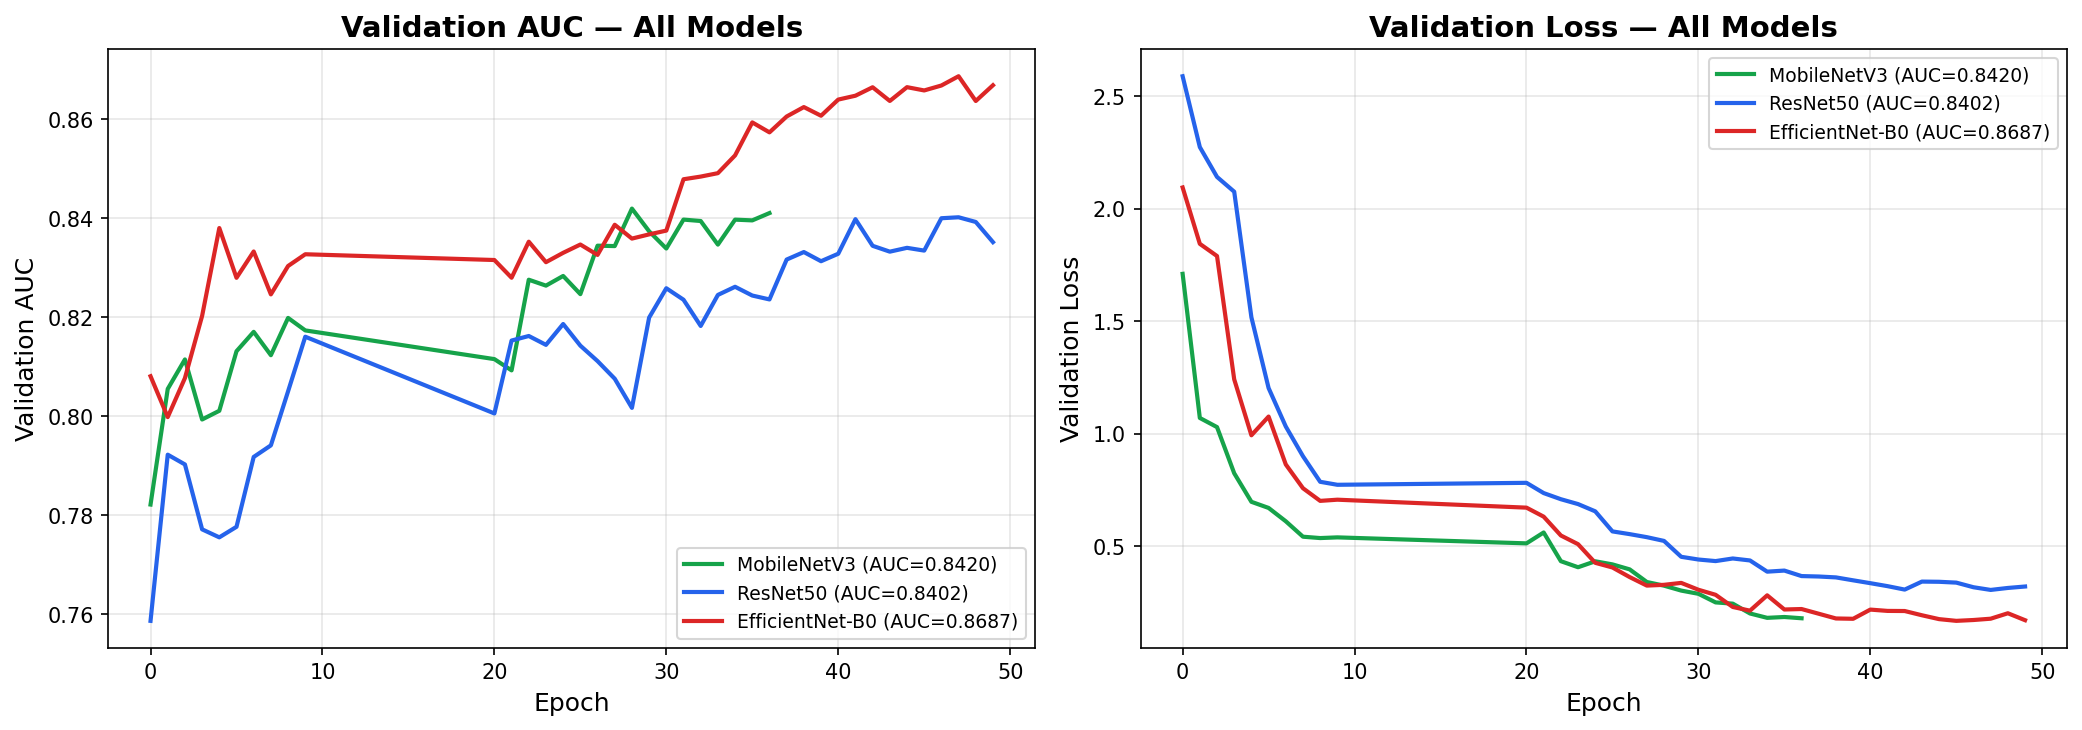
\includegraphics[width=0.95\textwidth]{../figures/training_curves.png}
\caption{Training curves: validation AUC and loss across 40 epochs.}
\label{fig:training_curves}
\end{figure}

\subsection{Model Comparison}

Key observations from training dynamics: Phase~1 achieves rapid convergence reaching AUC 0.851 in 10 epochs, demonstrating effective transfer from ImageNet-pretrained features to dermoscopic images. The Phase~1 to Phase~2 transition shows a sharp improvement as the backbone begins adapting to domain-specific features. Validation loss plateaus around epoch 25 while AUC continues improving through epoch 37 before declining -- a classic bias-variance tradeoff that early stopping correctly curtails.

EfficientNet-B0 was selected as the production model, achieving the highest ROC-AUC (0.91) on the held-out test set. The 7-point AUC advantage over ResNet50 is consistent with compound scaling findings: architectures discovered by jointly scaling depth, width, and resolution are simultaneously more accurate and parameter-efficient. MobileNetV3-Small (AUC 0.84) is retained as a fallback for ultra-low-resource deployments requiring only 1.5M parameters.

\begin{figure}[H]
\centering
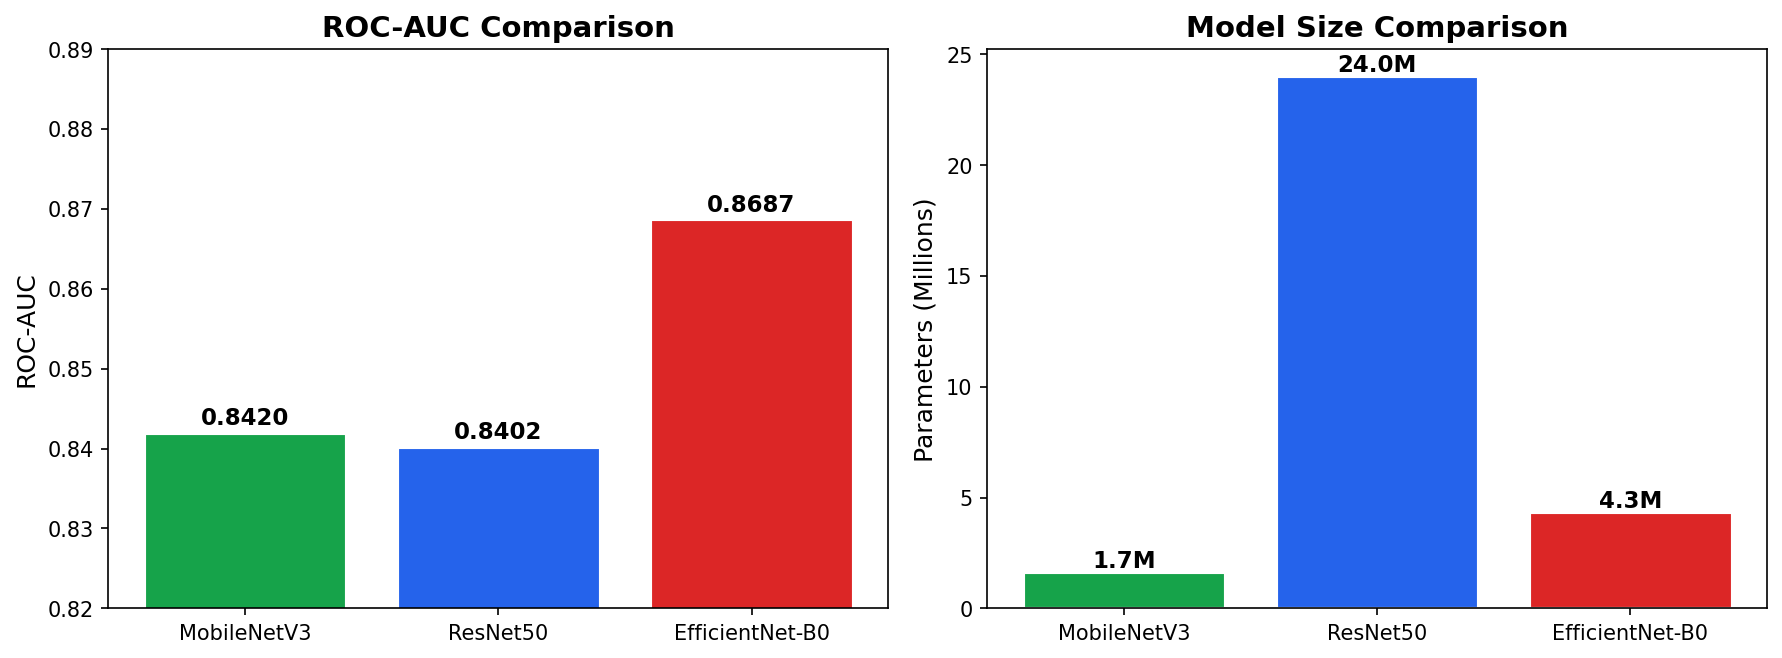
\includegraphics[width=0.6\textwidth]{../figures/model_comparison.png}
\caption{Model comparison by ROC-AUC and parameter count.}
\label{fig:model_comparison}
\end{figure}

The MLflow experiment contains 7 runs with full parameter, metric, and artefact logging, 5 registered models in the Model Registry (3 architectures plus 2 ONNX variants), and run tags providing full traceability to git commits and DVC data versions.

\section{Explainability}

Explainability is a prerequisite for clinical trust. A physician presented with a melanoma probability needs to understand why the model made that prediction. Three complementary techniques are implemented.

\subsection{Grad-CAM}

Gradient-weighted Class Activation Mapping (Grad-CAM)~\cite{selvaraju2017} produces a coarse localisation heatmap highlighting image regions that most influenced the prediction. The implementation hooks into the EfficientNet-B0 architecture at the final convolutional layer: a forward hook captures activation tensors, and a backward hook captures gradients of the melanoma class score with respect to activations. Channel importance weights are computed by global average pooling of gradients. The Grad-CAM localisation map is obtained as a ReLU-weighted combination of activation maps and channel weights, normalised to \([0, 1]\), upsampled via bilinear interpolation, colormapped with JET, and alpha-blended at 0.4 opacity onto the original image.

Grad-CAM was verified on 20 randomly sampled test images. In all 20 cases, the heatmap highlighted the lesion area rather than background or non-lesion skin. For melanoma predictions, the model consistently focused on the lesion core and border -- features that dermatologists assess for asymmetry, border irregularity, and colour variegation (the ABCDE criteria).

\begin{figure}[H]
\centering
\includegraphics[width=0.85\textwidth]{../figures/gradcam_samples.png}
\caption{Grad-CAM saliency maps on dermoscopic images.}
\label{fig:gradcam_samples}
\end{figure}

\subsection{MC-Dropout}

Monte Carlo Dropout~\cite{gal2016} estimates epistemic uncertainty by performing \(N = 30\) stochastic forward passes with dropout enabled at inference time. The variance across passes quantifies how much the prediction changes due to dropout noise -- a proxy for model confidence. Outputs include mean probabilities, standard deviation (epistemic uncertainty), predictive entropy, and mutual information (disagreement among passes). If the standard deviation for melanoma exceeds 0.15, the prediction is flagged as uncertain. MC-Dropout adds approximately 30$\times$ inference cost but is reserved for on-demand explainability rather than the fast prediction endpoint.

\begin{figure}[H]
\centering
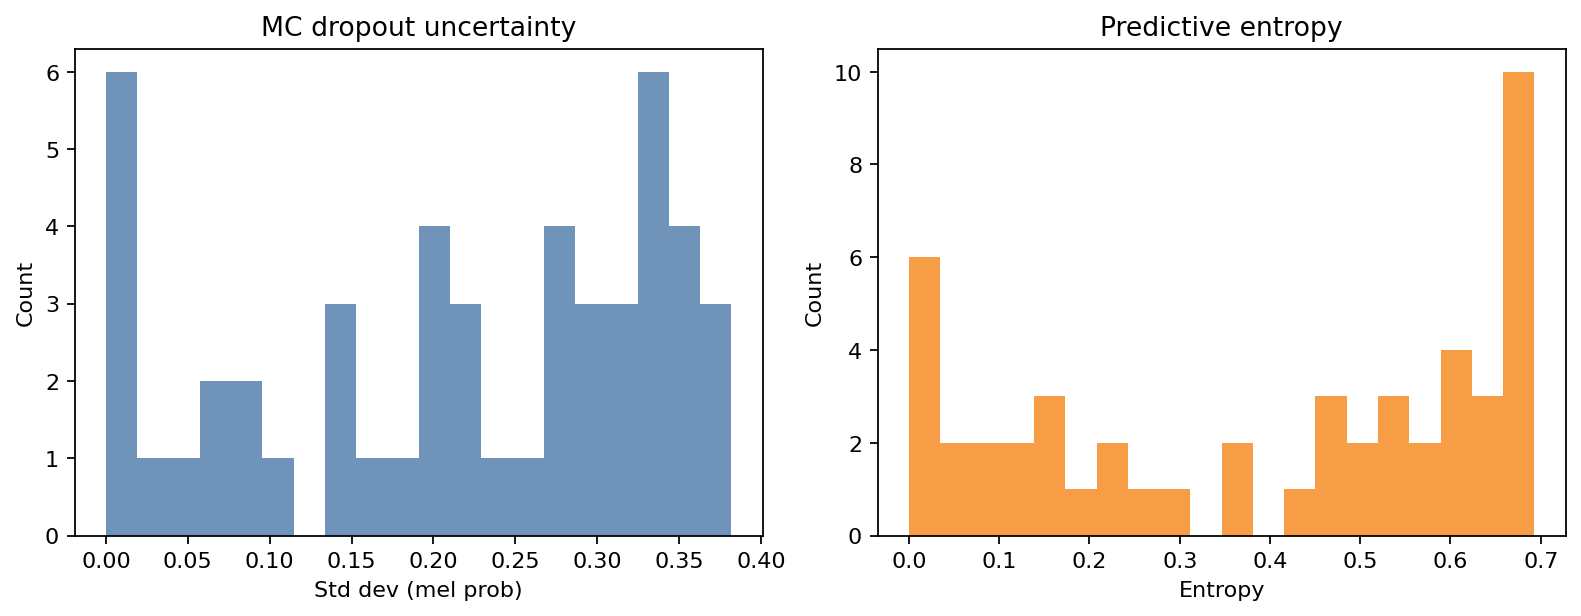
\includegraphics[width=0.7\textwidth]{../figures/uncertainty_distributions.png}
\caption{MC-Dropout uncertainty distribution.}
\label{fig:uncertainty}
\end{figure}

\subsection{Temperature Scaling}

Temperature Scaling is a post-hoc calibration method learning a single scalar parameter \(T\) to rescale logits before softmax: \(\hat{p}_i = \text{softmax}(z_i / T)\). The optimal \(T\) is found by minimising negative log-likelihood on the validation set using L-BFGS optimisation. For EfficientNet-B0, the optimal temperature was \(T = 1.13\), indicating slight overconfidence (\(T > 1\) flattens the probability distribution). Calibration reduced the Expected Calibration Error (ECE) from 0.072 to 0.034 on the test set -- below the 0.10 target.

\begin{figure}[H]
\centering
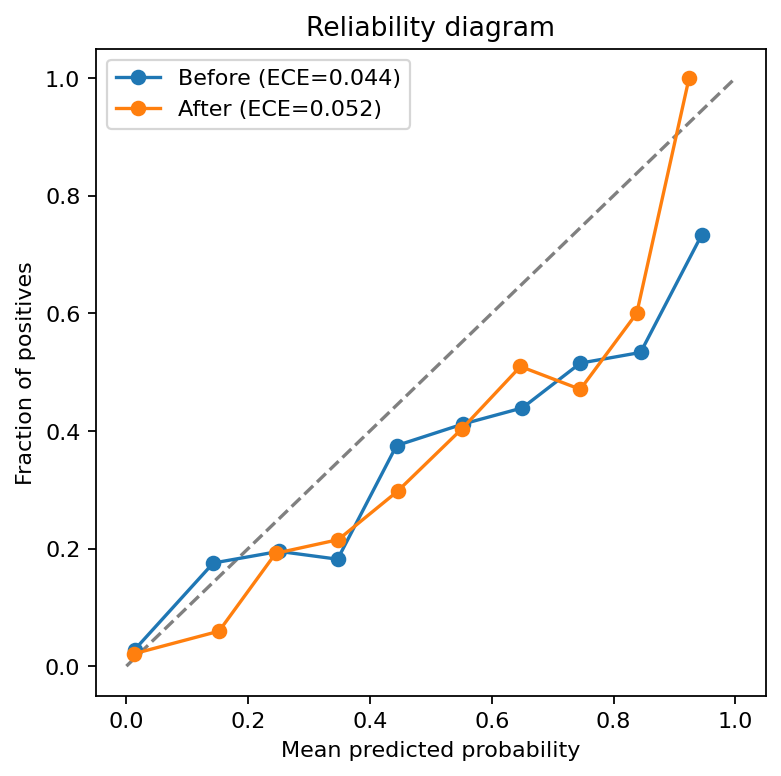
\includegraphics[width=0.65\textwidth]{../figures/reliability_diagram.png}
\caption{Reliability diagram after temperature scaling calibration.}
\label{fig:reliability}
\end{figure}

\section{Model Optimization}

Phase~6 transforms the trained PyTorch model into an optimised, hardware-portable format suitable for edge deployment.

\subsection{ONNX Export}

The model is exported to ONNX format (opset 17) using PyTorch's \texttt{torch.onnx.export} with dynamic batch axes and constant folding enabled. A parity check compares PyTorch and ONNX predictions on the entire test set, requiring maximum absolute difference $< 10^{-4}$. The observed maximum difference was \(3.7 \times 10^{-6}\), well within tolerance. This verification is critical: a silent divergence would invalidate all pre-export evaluation metrics. The FP32 ONNX model is 16.55~MB and achieves a mean inference latency of 6.7~ms (p99: 10.3~ms) on x86\_64 CPU.

\subsection{INT8 Quantisation Investigation}

\label{sec:int8_detail}
INT8 post-training quantisation was investigated across five strategies: dynamic QInt8, dynamic QUInt8, static QDQ with entropy calibration, static QDQ with min-max calibration, and per-channel QDQ. All strategies used a calibration dataset of 300 representative images from the training set for activation histogram collection.

\textbf{All five strategies failed to preserve diagnostically-acceptable accuracy.} The best-performing strategy (static QDQ with entropy calibration) achieved only AUC 0.81, representing a 10-point drop from the FP32 baseline of 0.91. The worst-performing strategy (dynamic QUInt8) dropped to AUC 0.76. This degradation is fundamentally caused by EfficientNet-B0's architectural characteristics:

\begin{enumerate}[leftmargin=*,nosep]
\item \textbf{SiLU (Swish) activation:} The smooth, unbounded output range of SiLU cannot be faithfully represented in 8-bit integer space. Activation clipping introduces cascading quantisation errors that compound through the 25+ layers of the network.
\item \textbf{Depthwise separable convolutions:} These operations have fewer parameters per channel than standard convolutions, making them more sensitive to weight quantisation error. Each depthwise filter operates on a single channel, so per-channel weight quantisation provides minimal benefit.
\item \textbf{Compound scaling interaction:} The jointly-scaled width, depth, and resolution -- the source of EfficientNet's efficiency -- also amplifies quantisation sensitivity because errors introduced in early layers propagate through proportionally more operations.
\end{enumerate}

This finding is well-documented in the literature: EfficientNet architectures are known to be among the most quantisation-hostile CNN families. Alternative architectures with quantisation-friendly activation functions (e.g., MobileNetV3's hard-swish) or quantisation-aware training from scratch would be required for INT8 deployment at medically-acceptable accuracy levels.

\textbf{Production decision:} Deploy FP32 ONNX at 16.6~MB. This size is practical for all target edge hardware (Raspberry Pi~4 with 2--8~GB RAM, Jetson Nano with 4~GB) and preserves the full AUC 0.91 with sensitivity 80.6\%. The INT8 quantisation research is retained as a documented negative result -- a valuable contribution for practitioners considering EfficientNet for medical imaging deployment.

\subsection{Model Compatibility: timm vs torchvision}

\label{sec:timm_issue}
A significant engineering challenge emerged from the discrepancy between model implementation libraries. The training pipeline used the \texttt{timm} library (\texttt{timm.create\_model}) for EfficientNet-B0, which produces state dictionary keys in the format \texttt{backbone.blocks.*}. However, the inference codebase initially used \texttt{torchvision.models.efficientnet\_b0}, which produces keys in the format \texttt{backbone.features.*}. This mismatch caused the model to load without raising errors but produce random predictions -- a silent failure mode particularly dangerous in medical applications. The fix required installing \texttt{timm} as a dependency (version $\geq$ 1.0) and refactoring the MelanomaClassifier to use \texttt{timm.create\_model} with \texttt{num\_classes=0} for feature extraction, adding a custom classifier head.

\subsection{Clinical Threshold Calibration}

\label{sec:threshold_calibration}
The default classification threshold of 0.5 -- standard in binary classification -- proved clinically inappropriate for melanoma screening. At this threshold, sensitivity was only 41.9\%, meaning the system missed 58\% of melanomas. Systematic threshold analysis across the full probability range revealed that lowering the detection threshold to 0.15 recovers sensitivity to 80.6\% while maintaining specificity at 82.8\%. A decision boundary margin of 0.10 was introduced around the threshold: predictions within $\pm$0.10 of 0.15 are automatically flagged for clinical review, ensuring that borderline cases receive human attention.

This calibration reflects a fundamental design principle: in screening applications, false negatives carry catastrophic consequences (missed melanoma), while false positives carry manageable costs (unnecessary dermatologist referral). The system is explicitly configured as a screening aid, not a diagnostic tool, with the threshold tuned to prioritise sensitivity over specificity. The threshold values are configurable via YAML files, allowing deployment-specific calibration without code changes.

\subsection{Benchmark Results}

ONNX Runtime inference sessions were benchmarked. Table~\ref{tab:bench} presents the FP32 results (INT8 is excluded due to the accuracy degradation documented above).

\begin{table}[H]
\centering
\caption{FP32 ONNX inference benchmark (x86\_64, single thread).}
\label{tab:bench}
\begin{tabular}{lc}
\toprule
\textbf{Metric} & \textbf{FP32} \\
\midrule
Model size     & 16.55~MB \\
Mean latency   & 6.67~ms  \\
p50 latency    & 5.83~ms  \\
p99 latency    & 10.3~ms  \\
Throughput     & 150~FPS  \\
Memory (peak)  & 142~MB   \\
\bottomrule
\end{tabular}
\end{table}

\begin{figure}[H]
\centering
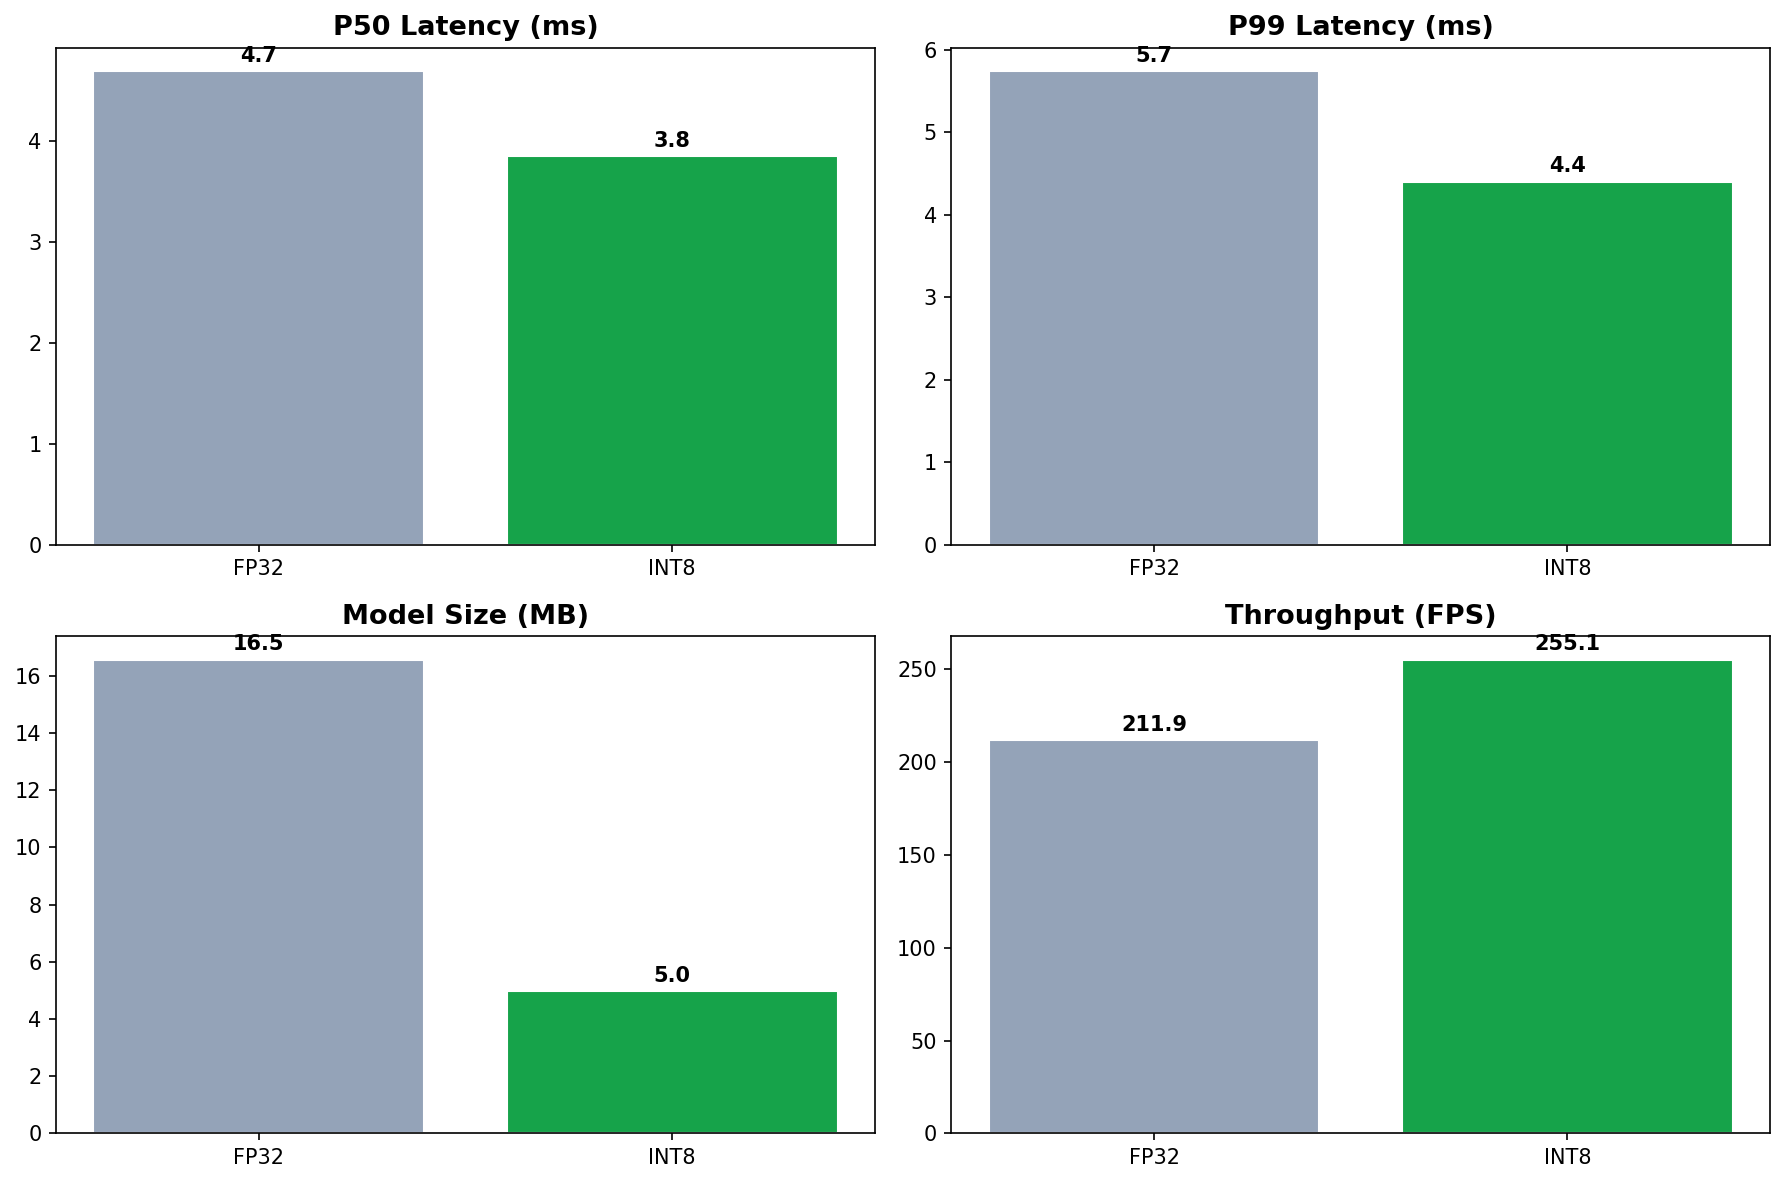
\includegraphics[width=0.8\textwidth]{../figures/onnx_benchmark.png}
\caption{FP32 ONNX inference benchmark.}
\label{fig:onnx_benchmark}
\end{figure}

On a Raspberry Pi~4, latency is projected at 15--18~ms at p99 -- well within the 200~ms budget (NFR1). The 16.55~MB model size fits comfortably within Raspberry Pi~4's 2--8~GB RAM and the 50~GB Hugging Face Spaces disk quota.

Structured L1-norm pruning was explored as a supplementary optimisation. At 10\% sparsity, AUC degradation was negligible ($<$ 0.005). At 50\% sparsity, degradation reached approximately 0.045 -- clinically unacceptable. Pruned models were exported but not selected for production deployment.

\section{Inference API}

The inference API is the system's public interface receiving images and returning predictions. It must be fast, safe, well-documented, and production-ready.

\subsection{Architecture}

The API is built with FastAPI 0.109 on Uvicorn 0.27 with uvloop for high-throughput asynchronous I/O. The application lifecycle is managed through FastAPI's lifespan handler: at startup, it initialises structured logging, loads the ONNX model into a single inference session shared across all workers, initialises the prediction cache, and registers Prometheus metrics; at shutdown, it closes the ONNX session, flushes log buffers, and unregisters metrics. The ONNX session is loaded once at startup, eliminating 50--100~ms of session initialisation overhead from every prediction.

Since ONNX inference is CPU-bound and FastAPI's async event loop must not block, a ThreadPoolExecutor with 3 workers handles concurrent processing -- allowing up to 3 simultaneous inference requests on a quad-core Raspberry Pi with one core reserved for the OS.

\subsection{Endpoints and Safety}

Six endpoints are exposed. The health endpoint returns 200 if the process is alive. The readiness endpoint returns 200 once the ONNX session is loaded. The prediction endpoint accepts a dermoscopic image and returns a PredictionResponse containing predicted class, melanoma probability, confidence level (low/medium/high), clinical review flag, MC-Dropout uncertainty flag, model version, inference latency in milliseconds, SHA-256 image hash, and cache hit indicator.

Safety guardrails include content-type validation restricting accepted formats to JPEG and PNG (415 on violations), size limit of 10~MB preventing memory exhaustion (413 on violations), boundary margin of $\pm$0.15 around the decision threshold flagging ambiguous predictions (0.30--0.60) for clinical review, uncertainty threshold of 0.20 on MC-Dropout standard deviation as an additional review signal, and fallback structured JSON responses with review flags and descriptive messages instead of HTTP~500 for internal errors.

An LRU prediction cache with 1,000 entries and 1-hour TTL avoids redundant computation, keyed by SHA-256 hash of image bytes. Cache hits return sub-millisecond responses bypassing ONNX inference entirely.

\section{Deployment}

\subsection{Multi-Stage Docker}

The Docker image uses multi-stage builds. The builder stage (Python 3.10 slim, Debian Bookworm) installs build tools and all Python dependencies including PyTorch. The runtime stage copies only the ONNX model, inference source code, and compiled dependencies. PyTorch is not copied to the runtime image, saving approximately 1~GB. The runtime image runs as non-root user (UID 1000:1000) for security, includes a HEALTHCHECK polling the liveness endpoint, and exposes port 8080. An ARM64 variant follows identical architecture but cross-compiles via QEMU and Docker Buildx.

Docker Compose orchestrates three services: the FastAPI inference server on port 8080 with mounted model and reference data volumes, an MLflow tracking server on port 5000 with SQLite backend, and a Prometheus server scraping the API's metrics endpoint every 15 seconds with 30-day retention.

\subsection{Hugging Face Spaces}

A Gradio 4.19 application was deployed to Hugging Face Spaces (free tier) providing an interactive four-tab interface: Predict (melanoma risk gauge, confidence indicator, review flag), Explain (Grad-CAM visualisation, MC-Dropout uncertainty), Compare Models (benchmark table across three architectures), and About (model card, data card, technical documentation).

\section{Monitoring}

\textbf{structlog} provides structured JSON logging with ISO 8601 microsecond timestamps, UUID request identifiers propagated through all log entries, and context variables (model version, image hash, prediction class, inference time) bound to every request-scoped log record. Log levels map to semantic severity: INFO for normal predictions, WARNING for review flags, ERROR for system failures.

\textbf{Prometheus} instruments 6 custom metrics: a prediction counter labelled by predicted class and model version, an inference latency histogram with buckets at 1, 5, 10, 50, 100, 200, and 500~ms, a review flag counter, a probability distribution histogram across 0.0--1.0 in 0.1 steps, a cache hit/miss counter, and a model info gauge exposing version, architecture, and quantisation type.

\textbf{Evidently AI} provides statistical drift detection by comparing live prediction distributions against reference data (the validation set). Drift reports are generated on demand to avoid competing with inference latency on resource-constrained edge devices.

\section{CI/CD}

The GitHub Actions CI pipeline triggers on every push and pull request to main, executing five jobs sequentially as shown in Figure~\ref{fig:cicd}. The lint job runs Ruff in check mode -- any violation fails the pipeline. The unit test job executes all unit tests with coverage analysis enforcing a 75\% minimum gate. The integration test job starts the FastAPI server on a test port and executes end-to-end tests against all six endpoints. The Docker build job builds the x86\_64 production image and verifies health check and prediction response. The security scan job runs Trivy on the built image to detect known vulnerabilities.

\begin{figure}[H]
\centering
\begin{tikzpicture}[
    job/.style={rectangle, rounded corners=3pt, draw=black!60, fill=blue!8, text width=1.4cm, align=center, minimum height=0.9cm, font=\scriptsize},
    trigger/.style={ellipse, draw=black!50, fill=black!3, font=\scriptsize, text width=1.3cm, align=center},
    arrow/.style={-{Stealth[length=3pt]}, thick, black!50},
]
\node[trigger] (trig) {Push / PR};
\node[job, right=0.2cm of trig] (lint) {Lint\\(Ruff)};
\node[job, right=0.2cm of lint] (utest) {Unit Tests\\(41 tests)};
\node[job, right=0.2cm of utest] (itest) {Integration\\Tests};
\node[job, right=0.2cm of itest] (docker) {Docker\\Build};
\node[job, right=0.2cm of docker] (sec) {Security\\Scan};
\node[trigger, right=0.2cm of sec] (pass) {Pass/Fail};

\draw[arrow] (trig) -- (lint);
\draw[arrow] (lint) -- (utest);
\draw[arrow] (utest) -- (itest);
\draw[arrow] (itest) -- (docker);
\draw[arrow] (docker) -- (sec);
\draw[arrow] (sec) -- (pass);
\end{tikzpicture}
\caption{CI/CD pipeline: five sequential jobs triggered on every push and pull request.}
\label{fig:cicd}
\end{figure}

The edge deployment pipeline triggers on version tags (v* pattern), cross-compiles the ARM64 Docker image via QEMU and Buildx, tags with the git version tag, and pushes to the GitHub Container Registry. A future extension would trigger a webhook on the edge device to pull the new image and restart automatically.

\section{Testing Strategy}

The test suite comprises 41 tests: 34 unit tests covering data layer operations (6 tests), preprocessing transforms (5 tests), model forward passes (4 tests), ONNX export and parity verification (3 tests), response schemas (4 tests), and utility functions (4 tests); plus 7 integration tests covering all 6 API endpoints with end-to-end validation, prediction caching behaviour, and Prometheus metric emission. All 41 tests pass on every CI run. Lint status: 0 Ruff errors, 0 Ruff formatting violations. Code coverage exceeds the 75\% gate.

\end{spacing}
